\part{Déroulement du stage}

\chapter{Projet OpenNebula}

\section{Premiers pas}

\paragraph*{}
Les premiers jours de mon stage ont été dédiés pour tester les logiciels OpenNebula et Xen sur une plateforme de test
composée d'un petit serveur accueillant OpenNebula, de deux machines utilisées comme hyperviseurs Xen et d'un NetApp.
Vivien, mon responsable de stage, avait déjà déployé un environnement de développement fonctionnel sur ces machines.

\paragraph*{}
Afin de prendre en main la plateforme, mon premier objectif a été de mettre à jour OpenNebula qui était en version 2.2 vers la version 3.0 Beta 1.
Cette version 2.2 a été modifiée par Vivien pour fonctionner avec un plugin qu'il a écrit pour ajouter le support de l'iSCSI pour déporter le stockage des images
disque des VMs sur le NetApp.
\\
Il m'a donc fallu comprendre puis adapter le travail de Vivien. J'ai ensuite effectué beaucoup de tests pour valider le fonctionnement
de la nouvelle solution et aussi en valider ma compréhension.
\\
Après avoir compris comment marchait OpenNebula de l'extérieur - en tant qu'utilisateur - j'ai téléchargé les sources et ai préparé un
environnement de développement pour éditer, compiler\footnote{Étape de construction de l'exécutable du logiciel à partir des sources},
débugger\footnote{Action de compiler et lancer un exécutable d'une certaine manière permettant de voir le fonctionnement interne de l'application
pendant son fonctionnement pour comprendre et corriger des bugs}, installer et tester le logiciel.

\section{Interface de commande}
\paragraph*{}
OpenNebula peut être piloté via plusieurs interfaces:
\begin{listi}
	\item une interface web appelé Sunstone. voir figure \ref{sunstone}.
	\item une CLI\footnote{\index{CLI}CLI: \emph{Command Line Interface}, interface en ligne de commande}. voir \ref{clione}.
	\item une API\footnote{\index{API}API: \emph{Application Programming Interface}, Interface de programmation} de type
		XML\footnote{XML: \emph{Extensible Markup Language}, langage de balisage extensible, est un format de de structuration de donnée générique.}/RPC
		\footnote{RPC: \emph{Remote Procedure Call}, appel de procédure distant, est un protocole réseau fait pour appeler des procédure au sein d'un programme
		travers d'un réseau}
\end{listi}

\subsection{La CLI d'OpenNebula}
\label{onecli}

\begin{figure}[H]
\centering
\begin{lstlisting}
oneadmin@opennebula:~$ onehost list
  ID NAME               RVM   TCPU   FCPU   ACPU   TMEM   FMEM   AMEM   STAT
   0 hyp1                 1    400    399    300     4G   2.7G   3.9G     on
   1 hyp2                 2    400    399    100     4G   1.2G   3.2G     on
\end{lstlisting}
\caption{L'affichage de la liste de tous les \emph{hosts}/hyperviseurs}
\end{figure}


\begin{figure}[H]
\centering
\begin{lstlisting}
oneadmin@opennebula:~$ onevm list
ID USER     GROUP    NAME         STAT CPU     MEM        HOSTNAME        TIME
 0 oneadmin oneadmin vm1          runn   1    256M            hyp2 08 03:36:24
 1 oneadmin oneadmin vm2          runn   4   2048M            hyp2 00 00:01:38
 2 oneadmin oneadmin vm3          runn   2    128M            hyp1 00 00:01:00
\end{lstlisting}
\caption{L'affichage de la liste des VMs}
\end{figure}



\subsection{L'interface web Sunstone}

\begin{figure}[H]
\centering
\subfloat[\emph{Dashboard} / Tableau de bord]{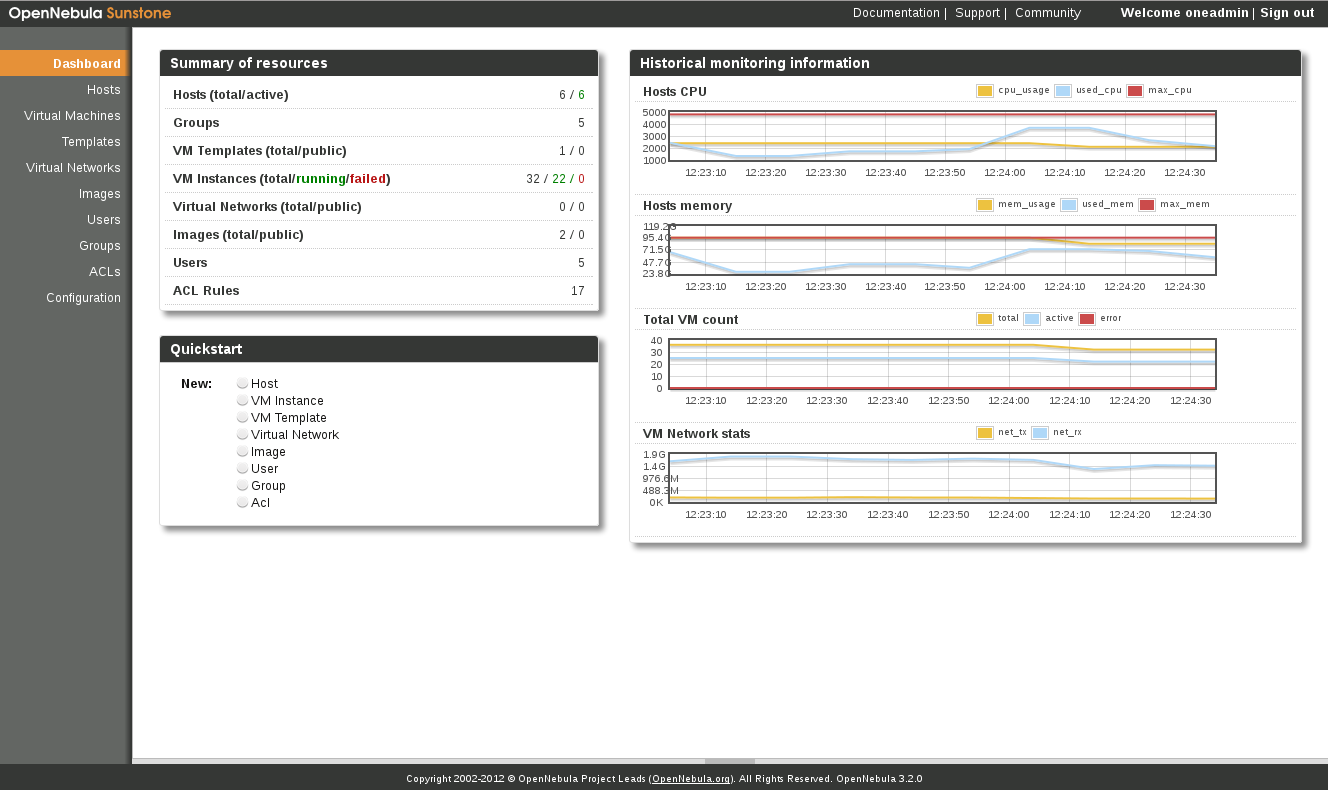
\includegraphics[width=0.5\textwidth]{resource/img/sunstone-dashboard}}
\subfloat[Création d'une VM]{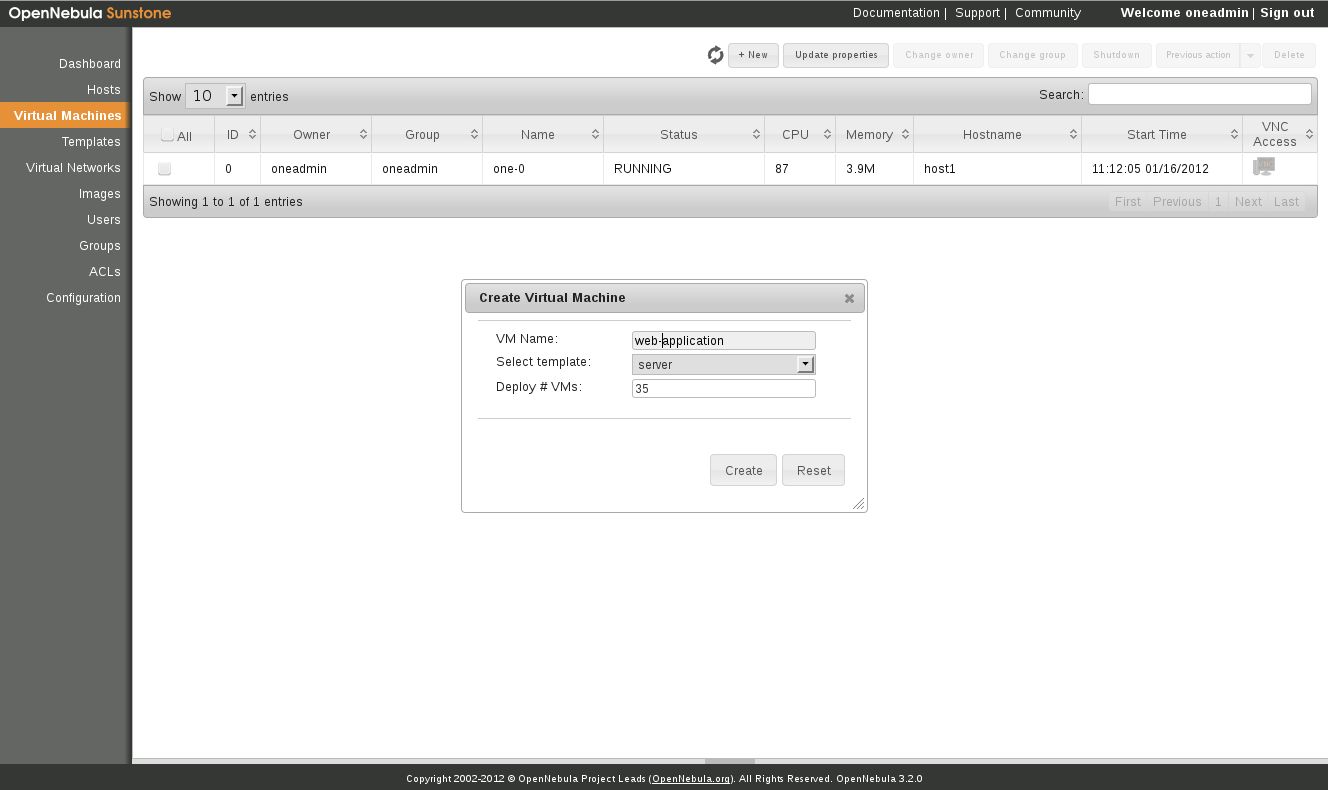
\includegraphics[width=0.5\textwidth]{resource/img/sunstone-createvm}}
\\
\subfloat[Création d'un template de VM]{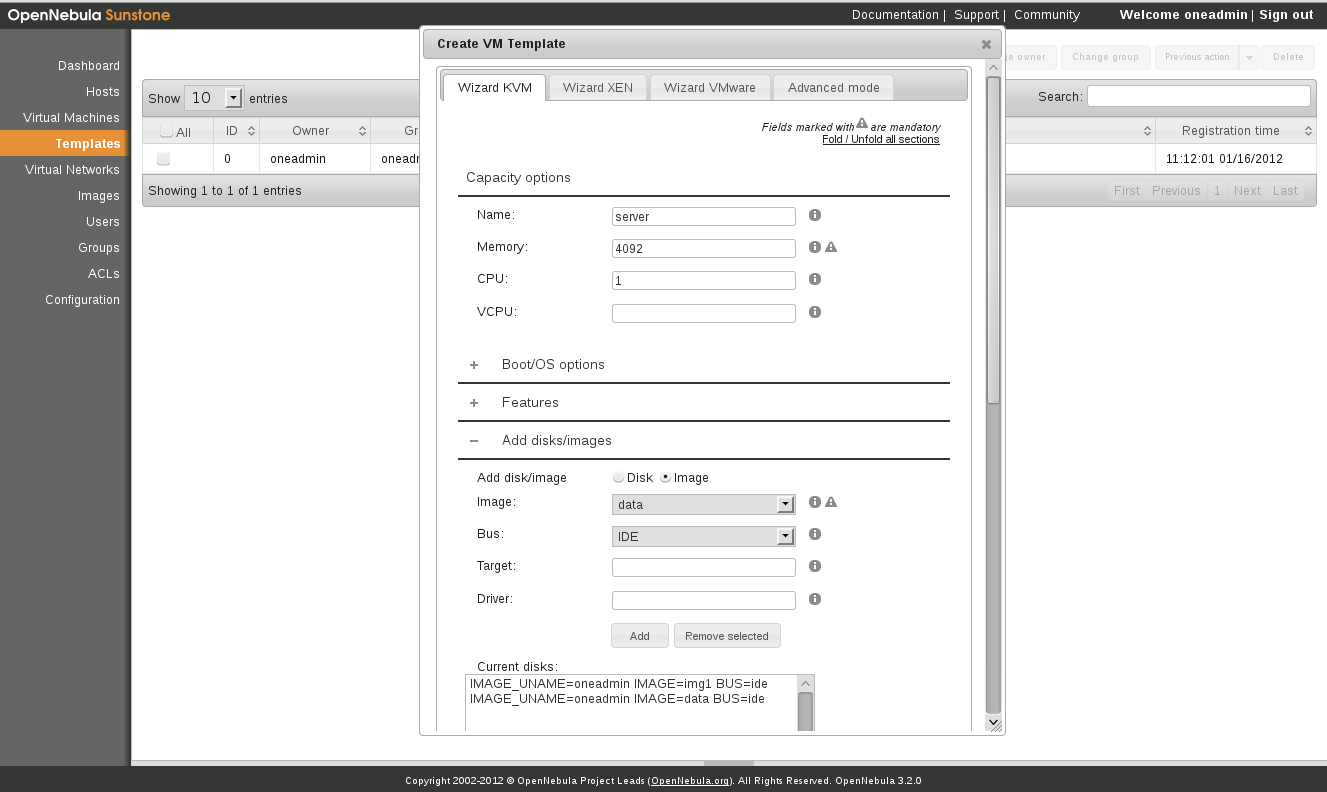
\includegraphics[width=0.5\textwidth]{resource/img/sunstone-createtemplate}}
\subfloat[Affichage de la liste des \emph{hosts}]{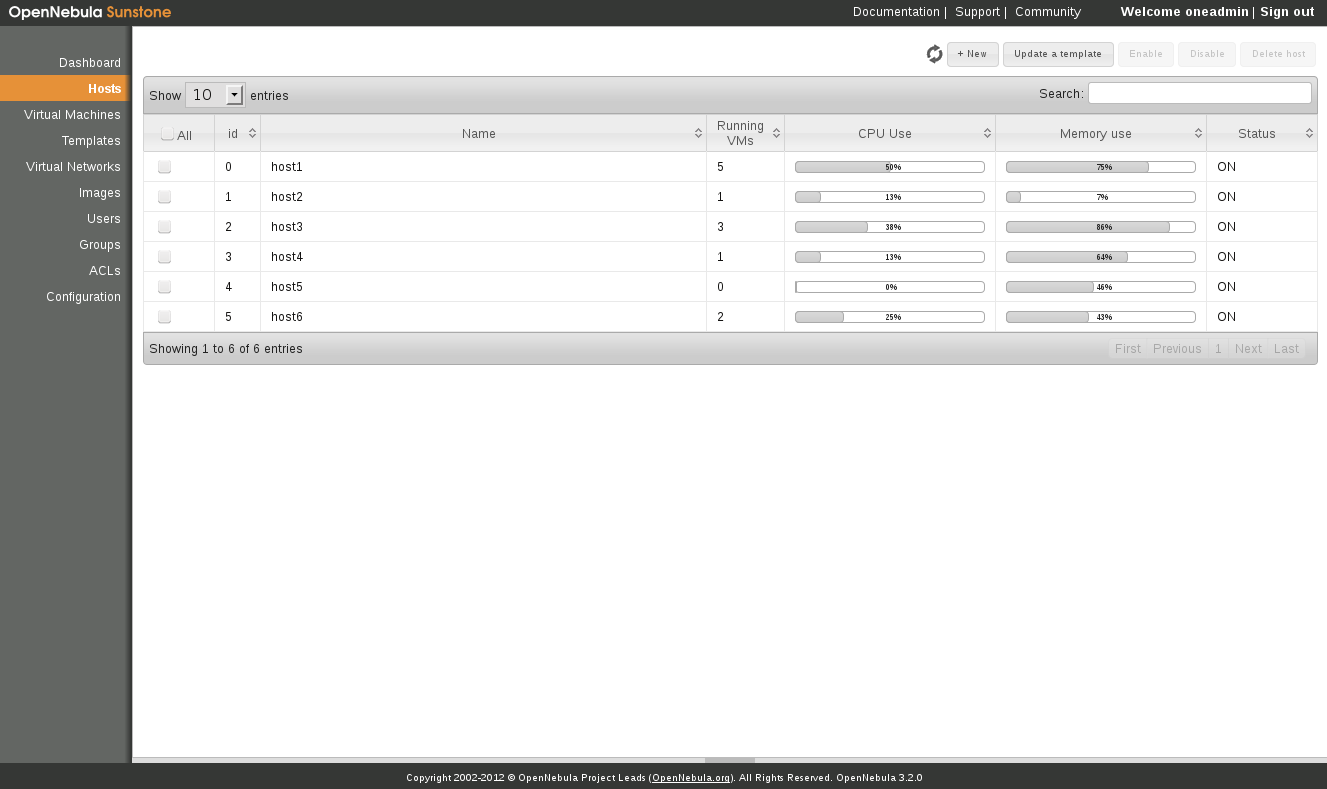
\includegraphics[width=0.5\textwidth]{resource/img/sunstone-hosts}}

\caption{L'interface web Sunstone d'OpenNebula}
\index{Sunstone}
\label{sunstone}
\end{figure}

\subsection{Architecture du code d'OpenNebula}
\paragraph*{}
Le code d'OpenNebula est designé comme une machine à état séparés en modules qui communiquent des ordres d'action de manière asynchrone.
\\
Chaque module tourne dans le contexte d'un \emph{thread} et utilise une file d'attente FIFO\footnote{FIFO: \emph{First In First Out}, est une structure de donnée où les données poussées à l'interieur
en premier sont celles qui en sortent en premier aussi} pour recevoir les messages des autres \emph{threads} de manière asynchrone.

\paragraph*{}
La machine à état d'OpenNebula est principalement axée autour des états des VMs et plus précisément autour du lien entre les VMs et les \emph{Hosts}.


\section{L'environnement}

\paragraph*{}
Pour l'ajout des fonctions de \emph{scale-in}, j'ai du en même temps regarder ce qui était techniquement possible au niveau de l'hyperviseur Xen qui
sera utilisé comme backend\footnote{Un backend est la partie basse d'une architecture utilisé pour éffectuer des actions à l'extérieur du logiciel.
Par opposition le frontend est la partie haute de l'architecture recevant les ordres de l'utilisateur et commandant les autres parties de l'architecture}
par OpenNebula pour créér les VMs sur un hyperviseur.

\paragraph*{}
En effet, en fonction des différentes versions du noyau Linux et de Xen, certaines fonctionnalités sont disponibles, indisponibles ou buggées.\\
J'ai donc fait un tableau LibreOffice Calc\footnote{Logiciel \emph{open source} concurrent de Microsoft\textsuperscript{\textregistered} Excel\texttrademark}
pour répertorier l'état de chaque fonctionnalité en fonction de toutes les combinaisons de versions possibles.
\\
Grâce à ce tableau, nous avons pu déterminer quelles étaient les fonctionnalités que nous allions utiliser puis par déduction quelles versions de logiciels nous
allions installer.

\paragraph*{}
Après avoir expérimenté avec la base de code d'OpenNebula nous avons fait des dessins d'architecture puis déterminé une procédure pour mettre en oeuvre ces
modifications.


\section{Nouvelle architecture}

L'objectif était de commencer par s'occuper des modifications de la gestion du stockage puis d'ajouter le support du \emph{scale in} qui est moins important.

\subsection{La gestion du stockage des images disque}
\paragraph*{}
Pour l'instant OpenNebula considère que les images disque des VMs sont soit stockées en local sur l'hyperviseur soit partagées sur un répertoire NFS
	\footnote{NFS: Network File System, est un système de fichier qui permet d'accèder à des fichiers via le réseau. Plusieurs clients peuvent accèder
	au mêmes fichiers en même temps. Ce système ressemble au protocole SMB de Microsoft\textsuperscript{\textregistered}}\index{NFS}.
Vivien à aussi écrit un plugin OpenNebula pour partager les images disque via l'iSCSI - plus performant que le NFS pour ce type d'utilisation.
\\
Dans tous les cas, OpenNebula n'a pas été \textsl{designé} pour gérer plusieurs serveurs de stockage et répartir les images disque sur ceux-ci.
\\
Les deux objets les plus importants manipulés par OpenNebula sont les \emph{Hosts} et les VMs. Un \emph{Host} est le nom utilisé par OpenNebula pour
designer un hyperviseur.
Un \emph{Host} contient donc zéro ou plusieurs VMs et une VM a forcément un et un seul \emph{Host} associé.


\paragraph*{}
Notre objectif serait de faire la même relation entre les images disques vs les serveurs de stockage et les VMs vs les \emph{Hosts}.
\\
OpenNebula n'a pour l'instant pas la notion de ce qu'est un serveur de stockage. Une image disque est juste un attribut d'une VM et n'a
pas de propriété faite pour désigner sur quel serveur de stockage elle se trouve.\\
De plus, par défaut, OpenNebula considère que l'image disque d'une VM ne contient aucune donnée importante et est supprimée aussitôt
que la VM est détruite.

\paragraph*{}
Nous avons donc créé dans le code d'OpenNebula un nouveau type d'objet appelé \emph{storage backend}, littéralement << object s'occupant du stockage >>.
Un \emph{storage backend} pourra être un NetApp, un serveur NFS ou un cluster Ceph\footnote{Ceph est un système de fichier distribué parallèle tolérant aux fautes.
Voir chapitre \ref{fsdpft}} par exemple. Une image disque devient donc principalement un attribut d'un
\emph{storage backend} et peut vivre et être manipulée indépendamment des VMs.


\paragraph*{}
Ce nouvel objet a nécéssité énormément de modifications au code source d'OpenNebula:
\begin{enumerate}
	\item Ajout de plusieurs modules pour gérer le cycle de vie d'un \emph{storage backend} et ses liens avec les autres objets du système.
	\item \textsl{Designer} un protocole de communication générique avec les \emph{drivers}/pilotes des \emph{storage backend}.
	\item L'écriture d'une architecture de gestion de plugin/driver pour communiquer avec le \emph{storage backend}.
	\item \textsl{Rédesigner} entièrement et réécrire le \emph{Transfert Manager} (Gestionnaire de transfert) car il n'était pas du tout assez flexible
		pour gérer les tranferts entre les différents \emph{storage backend}.
	\item Étendre le protocole XML/RPC et les outils de la CLI pour pouvoir administrer ces nouvelles fonctionnalités.
	\item Documenter les modifications.
	\item Écrire des tests unitaires pour vérifier qu'il n'y a pas de régressions introduites.
	\item Envoyer les modifications à la communauté pour qu'elles soient introduites et maintenues officiellement dans le projet.
\end{enumerate}

\section{Bilan}

\subsection{Le problème}

\paragraph*{}
Après environ un mois de programmation sur OpenNebula, j'ai commencé à avoir des doutes sur la faisabilité du projet sur la durée du stage et
aussi sur les chances que ces changements soit acceptés par la communauté.

\paragraph*{}
À ce stade, je commençais à avoir quelques parties de la nouvelle architecture qui fonctionnaient mais les changements apportés étaient très
conséquents et beaucoup plus dispersés que prévu. Nous pensions que le périmètre des modifications au projet serait beaucoup plus limité.\\
Voir un résumé des modifications apportées à OpenNebula en annexe \ref{modopennebula}.

\subsection{La remontée du problème}

\paragraph*{}
J'en ai donc parlé à mon tuteur de stage et nous avons réévalué la charge de travail restante et les chances que le projet soit accepté \emph{upstream}.
Nous avons aussi préparé une présentation de l'état actuel des choses et des alternatives possibles en cas d'abandon du projet OpenNebula pour
présenter au Chef de Projet d'Exploitation Kévin \textsc{Mazière} et au Directeur de Production Laurent \textsc{Alaguero}.

\paragraph*{}
Les alternatives possibles étaient soit d'écrire entièrement (\emph{from scratch}\footnote{littéralement: << depuis zéro >>}) un nouveau gestionnaire de
cloud correspondant parfaitement à notre besoin et seulement à notre besoin ou d'acheter des licences VMWare\textsuperscript{\textregistered} qui pourraient
convenir à notre besoin mais très onéreuses et en désaccord avec l'esprit de l'entreprise (préférence des logiciels Open-Source).

\subsection{La prise de décision}
\paragraph*{}
Suite à la réunion d'avancement du projet, il a été décidé de mettre en pause le développement sur OpenNebula et de lancer un
POC\footnote{\index{POC}POC: \emph{Proof Of Concept}, Preuve de concept} de la méthode de développement << \emph{from scratch} >> .



\chapter{Le projet H2O}
\index{H2O}
\paragraph*{}
H2O est le nom de code du projet de création d'un nouveau gestionnaire de cloud.
Grâce à notre expérience sur le projet OpenNebula, Vivien et moi avons pu très rapidement désigner une nouvelle architecture
simple et robuste, basée sur la philosophie du KISS\footnote{KISS: \emph{Keep It Stupid Simple}, << Garde ça simple, stupide >>}.


\section{Choix techniques}
\paragraph*{}
Nous avons choisi d'utiliser le langage de programmation Ruby pour le développement d'H2O. Ruby est un langage de très haut niveau
\footnote{Un langage de haut niveau est un langage de programmation dont la grammaire permet de programmer sans tenir compte des détails inhérents au
fonctionnement de l'ordinateur. Un langage de haut niveau permet de manipuler des concepts bien plus élaborés, mais empêche la gestion de certains détails.}
Ce langage est très réputé pour sa productivité et la << beauté >> du code que l'on peut écrire avec. Son principal défaut est sa grande lenteur d'exécution
mais ce n'est pas un problème pour notre projet.

\paragraph*{}
Notre architecture est -- tout comme OpenNebula -- séparée en plusieurs modules, mais à la différence de celui-ci nous avons choisi de faire que toutes les actions soient gérées
de manière séquencielle synchrone.\\ %Oui c'est un peut redondant mais c'est pour être sur que le lecteur comprenne.
Encore une fois ce type de fonctionnement n'est pas optimal au niveau des performances, mais nous avons estimé que si nous déployons pas plus d'une centaine de VMs à
l'heure ça ne devrait pas poser de problème.
Tout gérer de manière synchrone permet de simplifier drastiquement la machine à état du programme, la gestion des erreurs, la complexité globale du code et le déboggage
du programme.

\paragraph*{}
Un autre choix important que nous avons pris est de faire passer toutes les communications entre les modules par une base de donnée (BDD\index{BDD})
SQL\footnote{\index{SQL}SQL: \emph{Structured Query Language} est un langage permettant de faire des requêtes dans une base de donnée structurée} (MySQL ou SQLite).
Cela permet de ne pas avoir à créer de protocole de communication entre les différents modules et garantit qu'à tout moment en cas de panne système (coupure électrique
par exemple) l'état du cloud soit enregistré dans la BDD.

\section{Développement}

\paragraph*{}
Pour le développement nous avons avec Vivien créé un dépôt GIT\index{GIT}\footnote{GIT est un gestionnaire de version décentralisé. Ce logiciel permet de travailler à plusieurs
sur les sources d'un logiciel et de garder un historique de toutes les révisions des sources du logiciel. Ce logiciel est utilisé par les 1200 développeurs du noyau Linux}

\paragraph*{}
Nous avons travaillé à deux, Vivien et moi, à plein temps sur ce projet. C'était très intéressant et nous sommes très rapidement arrivés à une démo fonctionnelle avec une bonne
qualité de code.
\\
Voici les fonctionnalités que nous avons implémenté après trois semaines:
\begin{listi}
	\item Gestion des hyperviseurs : enregistrement, désenregistrement, monitoring, vérification du bon fonctionnement...
	\item Gestion des VMs: création, suppression, \emph{live-migration}, affichage des informations ...
	\item \emph{Live Migration} entre deux hyperviseurs
	\item Gestion indépendante des images disques et cartes réseau et archives d'OS
	\item \emph{Hotplug} de mémoire RAM et de VCPUs et nouvelles images disque
	\item Redimentionnement d'images disque à chaud
	\item Gestion indépendante des images disques
	\item Interface en CLI uniquement. Voir annexe \ref{CLIH2O}.
\end{listi}

\section{Bilan}

\paragraph*{}
Après trois semaines de développement intensif nous avons jugé que nous étions prêt à faire notre démonstration à M. Alaguero, M. Mazière et un responsable commercial
M. Simonin.

\paragraph*{}
La démonstration s'est bien passée et tout le monde était très satisfait de ce que nous avions réussi à développer.

\paragraph*{}
Le problème c'est que durant la période de développement, Vivien, mon tuteur de stage, nous a annoncé qu'il quitterait la société fin décembre. Il a eu une proposition très intéressante
qu'il a acceptée mais a déplacé le jour de son départ le plus tard possible, c'est à dire au 1\textsuperscript{er} janvier 2012.

\paragraph*{}
En attendant qu'une nouvelle personne puisse s'occuper de la maintenance de cette solution après le départ de Vivien et de moi même, il m'a été demandé de mettre en pause ce projet
et de revenir sur le projet de \emph{scale-in} d'OpenNebula comme solution complémentaire à H2O.


\chapter{Le projet OpenNebula \emph{phase 2}}

\section{Présentation}
\paragraph*{}
Une fois le projet H2O complété mais en attente de mainteneur, il a été jugé utile de profiter de mon expérience sur le code source d'OpenNebula pour lui ajouter
le support du \emph{scale-in}, moins compliqué à implémenter.

\paragraph*{}
Ce travail était déjà prévu à l'origine du stage mais était moins priotitaire que le support de multiple \emph{storage backend}.
L'ajout du \emph{scale-in} n'est pas dépendant de cet ancien travail mais toujours aussi utile.\\

\section{Développement}
\paragraph*{}
Le début du développement a commencé après le départ de Vivien et c'est Kévin qui a pris la responsabilité de devenir mon responsable de stage.
Je me suis basé sur la dernière version stable d'OpenNebula, la version 3.2.

\paragraph*{}
J'ai tout d'abord fait une liste très précise de tous les modules du code source à modifier et à écrire. Pour chacune de ces étapes, j'ai essayé de déterminer
la charge de travail à effectuer, les risques associés et alternatives en cas de problème.

\paragraph*{}
Voici un aperçu très simplifié du code source d'OpenNebula qui ne contient que les composants principaux que nous devons modifier pour ajouter le \emph{scale-in}: \ref{archionescalein}.

\begin{figure}[H]
\centering
\includegraphics[width=0.9\textwidth]{resource/graph/ONE}
\caption{Les composants de l'architecture d'OpenNebula qui seront modifiés pour le support du \emph{scale-in}\\}
Les flêches représentent le sens du passage des messages dans le cas de l'exécution d'une commande par un utilisateur.
\label{archionescalein}
\end{figure}


\paragraph*{}
Pour reprendre la programmation sur OpenNebula, il m'a fallu réinstaller l'environnement de développement d'OpenNebula et redéployer notre architecture de test.
Ensuite j'ai réussi très rapidement à me << replonger >> dans le code d'OpenNebula et à implémenter une permière version fonctionnelle mais incomplete du \emph{scale-in}.

\paragraph*{}
À ce stade du développement, j'avais quelques hésitations sur des questions de design. J'ai donc décidé de contacter la communauté OpenNebula pour les informer de l'existance
du projet et leur demander conseil.\\
J'ai tout d'abord cherché à parler avec les développeurs sur IRC\footnote{\index{IRC}IRC: \emph{Internet Relay Chat}, protocole de messagerie instantanée beaucoup utilisée
par les développeurs de projets open-source.} sur leur salon officiel mais il n'y avait que très peu de monde et on m'a conseillé d'envoyer un mail sur la \emph{mailling-list} du
projet.

\paragraph*{}
J'ai donc écris et j'ai eu une réponse très positive du \emph{Project Engineer} d'OpenNebula.\\
L'échange de mail est disponible en annexe \ref{mailone}.


\chapter{Autres travaux}

\section{La Conférence OpenStack}
\paragraph*{}
Le 21 septembre 2011, à peine plus de deux semaines après mon début de stage une conférence internationale sur le Cloud Computing s'est déroulée à Paris.
Normalement Vivien \textsc{Bernet-Rollande} et Kévin \textsc{Mazière} devaient participer à cette conférence mais Kévin n'a finalement pas pu venir. J'ai donc
 pris sa place.

\paragraph*{}
Vivien et moi nous sommes rendu à la conférence à Paris.
Il y avait une cinquantaine de participants et une dixaine de présentations réparties toute la journée avec un petit buffet.

\paragraph*{}
La conférence était organisée par Rackspace pour la promotion de leur solution OpenStack. Plusieurs partenaires au projet étaient présents:\\
Dell, Canonical (Société derrière le système d'exploitation Ubuntu), UShareSoft, eNovance et OW2...

\paragraph*{}
Les conférences étaient pour la plupart en anglais. Les informations que j'ai appris m'ont été très utiles pour la suite de mon stage.\\
C'est aussi lors du moment des questions sur OpenStack que nous avons pu demander directement à un des manageur principal du projet pourquoi les solutions actuelles de Cloud
étaient si peu adaptées à nos problématiques. Voir chapitre \ref{cloudissues}.


\section{Le Projet STERN}
\paragraph*{}
Mi-octobre Kévin \textsc{Mazière} a eu pour mission de trouver des idées innovantes de projet en rapport avec le Cloud Computing par le groupe \textsc{Systematic Paris Region}.

\paragraph*{}
Le groupe \textsc{Systematic Paris Region} a pour mission de financer publiquement des projets de R\&D français et européens. Si notre projet est retenu par ce comité, Alter Way
recevra des fonds pour développer le projet à condition que celui-ci soit rendu open-source.

\paragraph*{}
Ce projet pourait être intéressant pour Alter Way. L'entreprise pourrait ainsi profiter d'ingénieurs supplémentaire en R\&D dans son équipe.
Elle profiterai aussi de l'expérience acquise sur le projet en développement. Elle aurait une position privilégiée sur une technologie innovante.\\
Le projet est aussi intéressant pour la communauté du Cloud Computing au sens plus large car l'accès au logiciel ainsi que son code source serait disponible à tous.


\paragraph*{}
Vivien en vacances à ce moment là et Kévin étant très occupé, on m'a demandé d'aider à trouver des idées.
Je me suis donc beaucoup documenté sur les diverses technologies de stockage utilisées dans le Cloud et les divers type d'hyperviseur.
\\
Un plus était de trouver des idées en rapport avec des besoins directs d'Alter Way.


\subsection{Les technologies de stockage}
\label{fsdpft}
\paragraph*{}
Je me suis beaucoup renseigné sur les divers systèmes de fichier distribués parallèles à tolérance de panne.

\paragraph*{}
Un système de fichier distribué signifie qu'il est accessible par plusieurs clients en même temps.

\paragraph*{}
Ce type de système de fichier distribue les données sur plusieurs serveurs sur un réseau. L'avantage est qu'il est possible d'avoir d'énormes systèmes de fichier de plusieurs
Pétaoctets (plusieurs millions de Gigaoctets).\\
Les performances sont aussi très bonnes car la charge est répartie sur l'intégralité du cluster.

\begin{figure}[H]
\centering
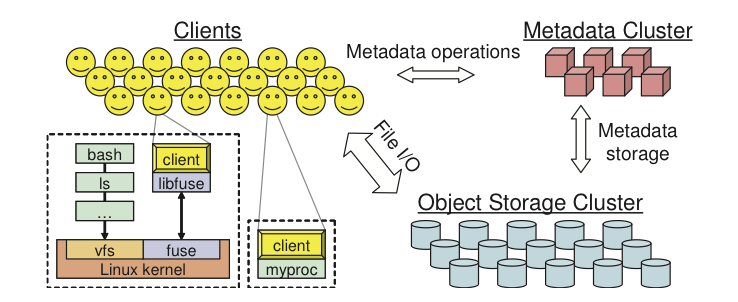
\includegraphics[width=0.9\textwidth]{resource/img/ceph-architecture}
\caption{Architecture générale de Ceph, un système de fichier distribué tolérant aux fautes}
\label{archionescalein}
\end{figure}

\paragraph*{}
Un autre avantage important de répartir les données sur plusieurs serveurs est qu'en cas de panne d'un ou plusieurs serveurs, si il y a suffisamment de redondance
de données dans le cluster. Il n'y aura pas d'interruption de service et le cluster répartira automatiquement la charge sur d'autres serveurs et redupliquera les données
des serveurs en pannes. C'est ce qu'on appelle la tolérance aux fautes (\emph{fault tolerance}).\\
Ensuite lors de l'ajout d'un nouveau serveur dans le cluster, le système de fichier placera automatiquement des données sur celui-ci et lui affectera une
partie de la charge du cluster.

\paragraph*{}
Pour résumer:
\begin{description}
	\item[Distribué] : accessible par plusieurs clients en même temps.
	\item[Parallèle] : répartie les données et la charge sur plusieurs serveurs.
	\item[Tolérant aux fautes]: peut perdre un ou plusieurs \emph{node}/serveurs et en rajouter à chaud de manière transparente et automatique.
\end{description}

\paragraph*{}
La première idée proposée au comité était de créer un nouveau système de fichier distribué, parallèle, tolérant aux fautes mais avec un design différent des implémentations actuelles
comme GlusterFS, Lustre ou encore Ceph.


\subsubsection{Les technologies de virtualisation par conteneur avec \emph{live-migration}}
\paragraph*{}
Une autre technologie qui pourrait être utile pour Alter Way en rapport avec le Cloud est la virtualisation par conteneur.

\begin{figure}[H]
\centering
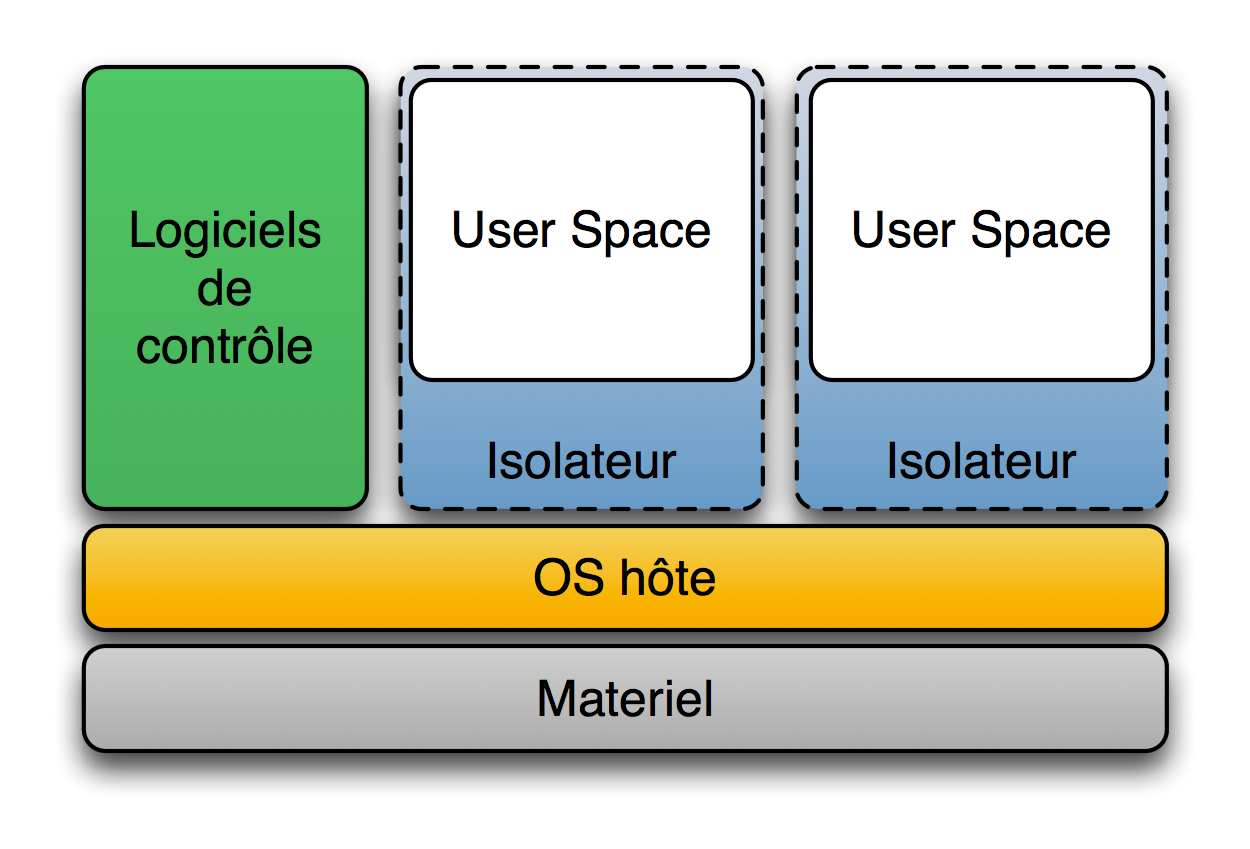
\includegraphics[width=0.6\textwidth]{resource/img/Diagramme_ArchiIsolateur}
\caption{Architecture de la virtualisation par conteneur/isolateur}
\end{figure}

\paragraph*{}
La virtualisation par conteneur est très différente de la virtualisation matérielle ou paravirtualisée car seule les applications sont virtualisées.
Toutes les applications tournent sur le même noyau mais celui-ci va simuler à chaque groupe de processus d'une VM qu'il est le seule à tourner sur
cette machine et ne lui permettra pas de communiquer avec les processus des autres VMs.

\paragraph*{}
Ce type de virtualisation permet d'utiliser la RAM de manière beaucoup plus efficiente que Xen par exemple car chaque VMs utilise le même noyau qui n'utilise
que la RAM nécéssaire pour chacun des processus des VMs. Sur Xen, il est nécéssaire d'allouer une quantité de RAM à chaque VMs, même s'il elle ne l'utilise pas complètement.
\\
Cela permet d'accumuler beaucoup plus de VMs sur un même serveur mais ces VMs auront moins de garanties de performances dans le cas ou toutes les VMs souhaitent utiliser
en même temps beaucoup de RAM, ce qui posera une très grosse perte de performance voir l'arrêt pur et simple d'une ou plusieurs VMs.

\paragraph*{}
Ce type de virtualisation est complémentaire au solution de virtualisation matérielle. La virtualisation matérielle est destinée aux clients exigeants ayant besoins de garanties
de performance. Elle sera facturée plus à cause du nombre plus restreint de VMs que l'on peut héberger sur un serveur.
\\
La virtualisation par conteneur permet d'avoir une offre moins chère pour les clients moins exigeants.

\paragraph*{}
La principale limitation des containeurs est qu'aucune technologie open-source existante ne permet de faire des \emph{live-migration}, essentielles pour correctement répartir
la charge entre les différents hyperviseurs d'un cluster de cloud.

\paragraph*{}
L'objectif du projet est donc d'ajouter le support de la live-migration sur la technologie de virtualisation la plus récente du noyau Linux: LXC
\footnote{LXC: \emph{\textbf{L}inu\textbf{X} \textbf{C}ontainer}}.


\subsubsection{La soumission des projets}
\paragraph*{}
D'autres idées ont été proposées à Kévin mais nous avons choisi de soumettre au comité les deux idées décritent précédemment.
\\
Après un premier retour du comité, il nous a été conseillé de concentrer nos efforts de spécification sur la deuxième idée -- plus réaliste au vu du budget/temps qui sera alloué au projet.

\paragraph*{}
Nous avons rédigé avec Kévin un cahier des charges et une présentation du projet de \emph{live-migration} de conteneur, alors nommé STERN\index{STERN}\footnote{STERN:
\textbf{S}ystème de \textbf{T}ransport d'\textbf{E}nvi\textbf{R}onnement \textbf{N}oyau, sterne est aussi le nom d'un oiseau.}

\paragraph*{}
Nous avons ensuite été convoqué à Paris dans les locaux de la société Open-Wide pour présenter notre projet au jury.
\\
Véronique \textsc{Torner} (Co-Présidente d'Alter Way), Hervé \textsc{Leclerc} (Directeur Technique), Kévin \textsc{Mazière} ainsi que moi-même nous sommes rendu sur place.

\paragraph*{}
Le jury était composé d'une quinzaine de personnes. Kévin a fait la présentation du projet et j'ai répondu aux questions techniques du jury. Véronique \textsc{Torner}
et Hervé \textsc{Leclerc} répondaient aux questions relatives à l'entreprise Alter Way.
\\
La présentation s'est bien passée et il y a eu des échanges de question-réponses très intéressants.


\subsubsection{Résultat}
\paragraph*{}
Deux semaines après la présentation nous avons reçu un mail du groupe Systematic nous informant que notre projet a été choisi par le jury!\\
Une copie du mail est disponible en annexe \ref{mailstern}.

\paragraph*{}
Malheureusement pour des raisons budgétaires et organisationnelles non prévues, le projet n'a pas eu de suite.
%
% \section{Déployement de Bacula sur FreeBSD et ZFS}
%
% \begin{pygmented}{c}
% void main(int argc, char* argv[])
% {
% 	printf("hello");
% 	return 0;
% }
% \end{pygmented}



\cite{test}
